\section{Модель}

\begin{quote}
\itshape{\large Мультитенантность} --- элемент архитектуры программного обеспечения, где единый экземпляр приложения, запущенного на сервере, обслуживает множество организаций-клиентов. Мультитенантность противопоставляется архитектуре из множественных экземпляров (англ. multiinstance), где для каждой организации-клиента создаются отдельные программные экземпляры. В мультиарендной архитектуре программные приложения работают одновременно с несколькими конфигурациями и наборами данных нескольких организаций, а каждая организация-клиент работает со своим экземпляром виртуального приложения, видя только свою конфигурацию и свой набор данных.
\end{quote}

%\begin{quote} Это абзац с отступами 1 см по бокам.
%    \begin{quote} А у этого отступы уже 2 см.
%    \end{quote}
%\end{quote}

%\rule{6cm}{0.4pt}\\[8pt]

\vspace{6pt}

\subsection{Схема инфраструктуры}
Для каждого разрабатываемого приложения известны сценарии его использвания и способы предоставления услуг. В данном случае, финальным результатом будет являться веб-приложение типа SaaS\footnote{%
	SaaS (англ. software as a service - программное обеспечение как услуга) --- одна из форм облачных вычислений, модель обслуживания, при которой подписчикам предоставляется готовое прикладное программное обеспечение, полностью обслуживаемое провайдером. Поставщик в этой модели самостоятельно управляет приложением, предоставляя заказчикам доступ к функциям с клиентских устройств, как правило через мобильное приложение или веб-браузер.
}. В качестве точки входа выступает сслыка в приложение для каждого клиента очередной организации. После этого каждому пользователю доступна площадка, в которой он может хранить различные файлы-модели, полученные в САПР приложениях, включая любую доументацию. На уровне организации доступна единая область памяти, способная быть ограниченной для любого члена организации. 

В итоге получаем информационную систему с возможностью изолированно обслуживать пользователей из разных организацией (т.е. независимых подписчиков SaaS) в рамках одного сервиса. Основным здесь является соблюдение изолированности подписчиков друг от друга. Действительно, клиенты не обрадуются, если данные, которые они хранят в SaaS приложении, будут доступны при поиске для других клиентов. Это явное нарушение изолированности.

Для реализации можно взять один сервер, одну операционную систему, одну базу данных. Механизм изоляции будет осуществляться с помощью особого хранения данных в таблицах БД и записью файлов в общую файловую сисему, а так же обработкой и перенаправлением web-запросов от клиентов на микросервисы.

Для достижения поставленных целей можно рассмотреть слудующую архитектуру сервера:

\begin{center}
	\begin{tabular}[t]{|c|p{15em}|}
		\hline
			ДНС-сервер\\
		\hline
			Прокси-сервер\\
		\hline
			Backend\\
		\hline
			БД\\
		\hline
			Файловое хранилище\\
		\hline
			Средства инфраструктуры\\
		\hline
	\end{tabular}
\end{center}

Каждый уровенень выполняет определенную роль. В совокупности c развитыми средствами автоматизации инфрастуктуры они реализуют целостную структуру информационной системы приложения. Далее будут рассмотрена каждый из них.

\subsection{Уровень ДНС-сервера}

\begin{quote}
\itshape{\large Доменное имя} --- основа для имени сайта, с помощью которой можно попасть на его ресурс.\\
\itshape{\large Доменная зона} --- совокупность доменных имён определённого уровня, входящих в конкретный домен.\\
\itshape{\large Делегирование} --- это передача контроля над частью доменной зоны другой ответственной стороне.
\end{quote}

\begin{figure}[H]
\centering
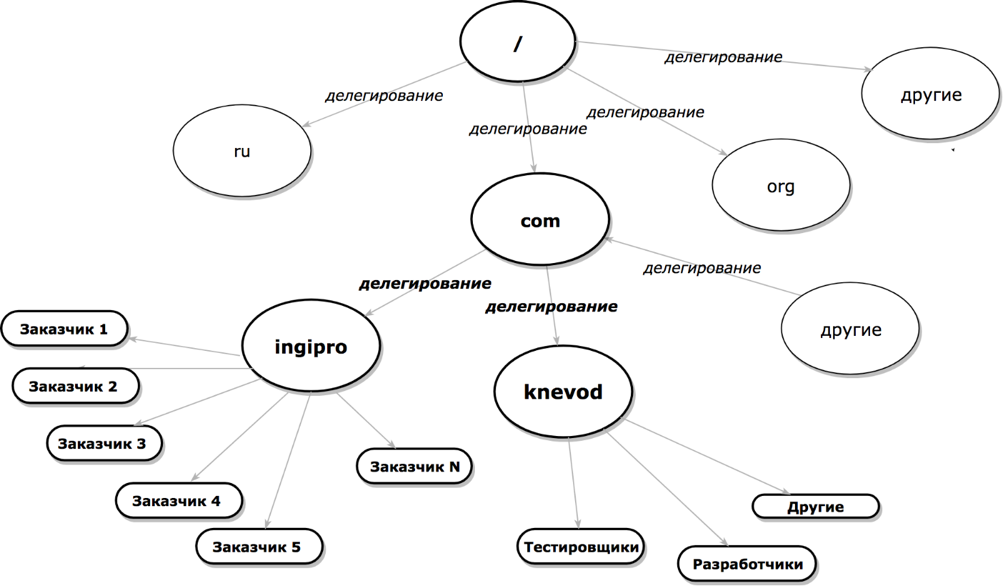
\includegraphics[scale=0.9]{dns.png}
\caption{Иерархия доменных имен}
\label{img:domains}
\end{figure}

ДНС\footnote{%
	DNS (англ. Domain Name System «система доменных имён») — компьютерная распределённая система для получения информации о доменах. Чаще всего используется для получения IP-адреса по имени хоста (компьютера или устройства), получения информации о маршрутизации почты, обслуживающих узлах для протоколов в домене.
} сервер в данной ситуации играет важную роль. На уровне доменных имен происходит разделенный досуп к инфрмационной системе. Это самый верхний уровень, который помогает реализовать множество точек входа в систему. Для того, чтобы добавить еще одного польователя, необходимо будет добавить в доменную зону новое имя, выделяемое для заказчика.

Так, например, если информационная система доступна по имени ingipro.com, то дабавив имя new-company в зону и получив адрес {\bfseries new-company.ingipro.com}, мы можем назначить клиенту этот адрес. Остальной механизм валидации осуществляется на следующих уровнях. 

В данном проекте используется Bind в качестве ДНС-сервера.

\subsection{Уровень Прокси-сервера}

На роль Прокси-сервера\footnote{%
	Прокси-сервер (от англ. proxy — «представитель», «уполномоченный») — промежуточный сервер в компьютерных сетях, выполняющий роль посредника между пользователем и целевым сервером, позволяющий клиентам как выполнять косвенные запросы (принимая и передавая их через прокси-сервер) к другим сетевым службам, так и получать ответы.
} возлагается много задач. Среди них:
\begin{itemize}
\item Обработка запрашиваемого адреса с целью перенаправления на другой адрес
\item Фильтрация и перенаправление запросов на уровень Backend
\item Выдача специальных ресурсов для запрашиваемого доменного уровня
\item Выдача статических ресурсов на сторону клиента
\end{itemize}

На этом уровне Веб-сервер\footnote{%
	Веб-сервер --- сервер, принимающий HTTP-запросы от клиентов, обычно веб-браузеров, и выдающий им HTTP-ответы, как правило, вместе с HTML-страницей, изображением, файлом, медиа-потоком или другими данными.
} Nginx, выступающий в роли Прокси-сервера, принимает HTTP-запросы от клиентов, перенаправляет их на необходимые микросервисы, которые в свою очередь реализуют основную логику работы разрабатываемого приложения. Далее возвращает в ответ HTTP-ответ с необходимым содержимым для отображения графического дизайна и данных в браузере клиента.


\subsection{Уровень Backend}

Backend\footnote{Backend --- программно-аппаратная часть сервиса. Набор приложений сервиса, работающих на стороне сервера.} является основной логической частью веб-приложения. Его архитектура бывает монолитной и микросервисной. В текущем проекте реализуется микросервисная архитекрура, состоящая из отдельных приложений, выполняющих специальные задачи. Так, например, существует микросервис, отвечающий за авторизацию пользователя в системе; микросервис, отвечающий за передачу файловых данных клиенту; микросервис, в основную задачу которого входит хранение множества атрибутов клиента; микросервис, отвечающий за отрисовку графических данных и так далее\dots

Каждый микросервис работает на специально выделенном сетевом порту сервера. В зависимости от поступившего от клиента HTTP-запроса происходит перенаправление на конкретный микросервис через сетевой порт. Во время работы Backend оперирует базой даных и файлами, располагающихся на жестком диске. Так проиходит обмен между уровнями инфраструктуры.
 
\subsection{Уровень Базы данных}

Огромное количество информации пользователей хранится в базе данных. Для ее управления используется СУБД\footnote{СУБД --- Система управления базой данных} PostgreSQL. Через нее микросервисы получают данные пользователей, хранящиеся в таблицах. Для достижения принципа мультитенантности реализуется следующий подход: пусть выделенная экосистема для клинета, называется new-company (по имени домена). Экосистема\footnote{Изолированное информационное пространство клиента для работы с сервисами приложения. Любые данные хранимые в экосистеме, связаны только с ней и клиентом на всех уровнях модели сервера.} в БД представляется двумя таблицами {\ttfamily attr\_new-company}, {\ttfamily entity\_new-company} и одной последовательностью {\ttfamily entity\_seq\_new-company}. Каждая заводимая экосистема хранит три объекта базы данных, которые относятся только к ней. Таким образом изолируются данные клиентов на уровне БД.

\subsection{Уровень файлового хранилища}

Уровень файлового хранилища представляет из себя часть файловой системы, находящейся на локальном или удаленном диске. Тут хранятся гораздо более тяжелые данные мультимедийного характера: документы, изображения, чертежи, аудио и видео записи. Область файлового хранилища закрыта от системных пользователей на уровне ОС и доступ туда имеют только программы, относящиеся к сервису. Как было сказано выше, любые данные Экосистемы имеют отношение только к ней самой. Поэтому в способ хранения информации Экосистемы выглядит слудующим образом:
\begin{figure}[H]
%\centering
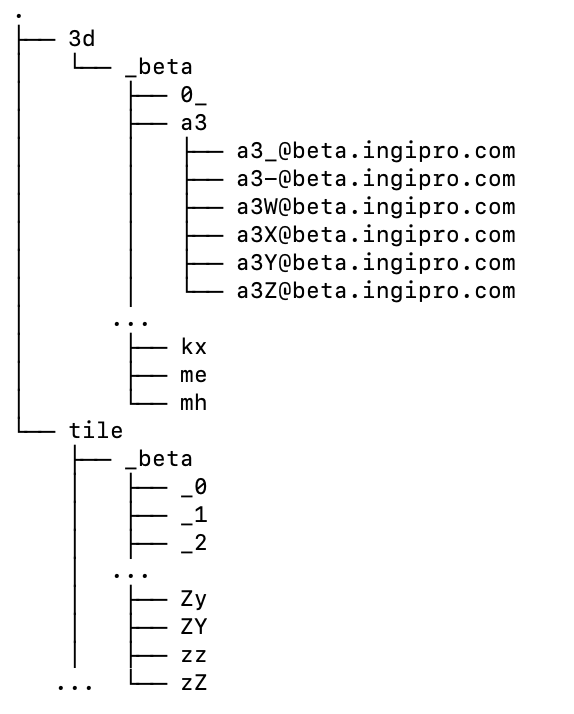
\includegraphics[scale=0.9]{tree.png}
\caption{Структура файлового хранилища}
\label{img:tree}
\end{figure}

На (рис. \ref{img:tree}) показан пример для экосистемы под названием {\ttfamily \_beta}. Таким структурированным образом хранится информация любых документов, изображений и моделей систем САПР в виде отдельных тайлов.

\subsection{Средства инфраструктуры}

Все вышеописанные уровни модели сервера реализуют определенные задачи. Все вместе они формируют программную систему, которая предлагается как конечный продукт. За реализацию каждого уровня отвечает определенный разрабочик или команда разработчиков. Они используют собственные средства, обычно не совместимые с продуктами других уровней. Это разные языки программирования, сетевые интерфейсты, логика работы приложения, конфигурационные файлы. Часто для внедрения новой версии, например backend, требуется внесения изменений в веб-сервере или DNS-сервере. Это несет некоторые трудности, так как требует работы нескольких команд или людей. 

Для решения подобных проблем выступают различные сервисы непреревной интеграции и доставки. Они оперируют специальными агентами, которые выполняют конкретные задачи при замене версий. Главной целью средств инфраструктуры выступает автоматизация процессов обновления, останова и запуска. Это всегда уникальные решения, которые адаптированы для текущей системы.